% Created by tikzDevice version 0.12.3 on 2020-01-31 10:11:36
% !TEX encoding = UTF-8 Unicode
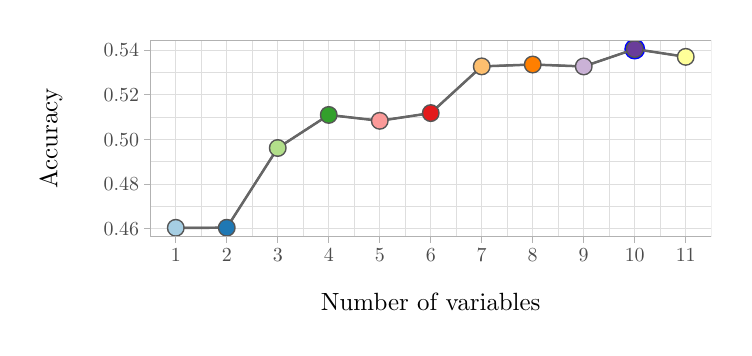
\begin{tikzpicture}[x=1pt,y=1pt]
\definecolor{fillColor}{RGB}{255,255,255}
\path[use as bounding box,fill=fillColor,fill opacity=0.00] (0,0) rectangle (251.50,108.41);
\begin{scope}
\path[clip] (  0.00,  0.00) rectangle (251.50,108.41);
\definecolor{drawColor}{RGB}{255,255,255}
\definecolor{fillColor}{RGB}{255,255,255}

\path[draw=drawColor,line width= 0.5pt,line join=round,line cap=round,fill=fillColor] (  0.00,  0.00) rectangle (251.50,108.41);
\end{scope}
\begin{scope}
\path[clip] ( 44.29, 32.86) rectangle (247.00,103.91);
\definecolor{fillColor}{RGB}{255,255,255}

\path[fill=fillColor] ( 44.29, 32.86) rectangle (247.00,103.90);
\definecolor{drawColor}{gray}{0.87}

\path[draw=drawColor,line width= 0.1pt,line join=round] ( 44.29, 43.89) --
	(247.00, 43.89);

\path[draw=drawColor,line width= 0.1pt,line join=round] ( 44.29, 60.02) --
	(247.00, 60.02);

\path[draw=drawColor,line width= 0.1pt,line join=round] ( 44.29, 76.14) --
	(247.00, 76.14);

\path[draw=drawColor,line width= 0.1pt,line join=round] ( 44.29, 92.27) --
	(247.00, 92.27);

\path[draw=drawColor,line width= 0.1pt,line join=round] ( 44.29, 32.86) --
	( 44.29,103.91);

\path[draw=drawColor,line width= 0.1pt,line join=round] ( 62.72, 32.86) --
	( 62.72,103.91);

\path[draw=drawColor,line width= 0.1pt,line join=round] ( 81.15, 32.86) --
	( 81.15,103.91);

\path[draw=drawColor,line width= 0.1pt,line join=round] ( 99.58, 32.86) --
	( 99.58,103.91);

\path[draw=drawColor,line width= 0.1pt,line join=round] (118.01, 32.86) --
	(118.01,103.91);

\path[draw=drawColor,line width= 0.1pt,line join=round] (136.43, 32.86) --
	(136.43,103.91);

\path[draw=drawColor,line width= 0.1pt,line join=round] (154.86, 32.86) --
	(154.86,103.91);

\path[draw=drawColor,line width= 0.1pt,line join=round] (173.29, 32.86) --
	(173.29,103.91);

\path[draw=drawColor,line width= 0.1pt,line join=round] (191.72, 32.86) --
	(191.72,103.91);

\path[draw=drawColor,line width= 0.1pt,line join=round] (210.14, 32.86) --
	(210.14,103.91);

\path[draw=drawColor,line width= 0.1pt,line join=round] (228.57, 32.86) --
	(228.57,103.91);

\path[draw=drawColor,line width= 0.1pt,line join=round] (247.00, 32.86) --
	(247.00,103.91);

\path[draw=drawColor,line width= 0.2pt,line join=round] ( 44.29, 35.83) --
	(247.00, 35.83);

\path[draw=drawColor,line width= 0.2pt,line join=round] ( 44.29, 51.96) --
	(247.00, 51.96);

\path[draw=drawColor,line width= 0.2pt,line join=round] ( 44.29, 68.08) --
	(247.00, 68.08);

\path[draw=drawColor,line width= 0.2pt,line join=round] ( 44.29, 84.21) --
	(247.00, 84.21);

\path[draw=drawColor,line width= 0.2pt,line join=round] ( 44.29,100.33) --
	(247.00,100.33);

\path[draw=drawColor,line width= 0.2pt,line join=round] ( 53.51, 32.86) --
	( 53.51,103.91);

\path[draw=drawColor,line width= 0.2pt,line join=round] ( 71.94, 32.86) --
	( 71.94,103.91);

\path[draw=drawColor,line width= 0.2pt,line join=round] ( 90.36, 32.86) --
	( 90.36,103.91);

\path[draw=drawColor,line width= 0.2pt,line join=round] (108.79, 32.86) --
	(108.79,103.91);

\path[draw=drawColor,line width= 0.2pt,line join=round] (127.22, 32.86) --
	(127.22,103.91);

\path[draw=drawColor,line width= 0.2pt,line join=round] (145.65, 32.86) --
	(145.65,103.91);

\path[draw=drawColor,line width= 0.2pt,line join=round] (164.07, 32.86) --
	(164.07,103.91);

\path[draw=drawColor,line width= 0.2pt,line join=round] (182.50, 32.86) --
	(182.50,103.91);

\path[draw=drawColor,line width= 0.2pt,line join=round] (200.93, 32.86) --
	(200.93,103.91);

\path[draw=drawColor,line width= 0.2pt,line join=round] (219.36, 32.86) --
	(219.36,103.91);

\path[draw=drawColor,line width= 0.2pt,line join=round] (237.79, 32.86) --
	(237.79,103.91);
\definecolor{drawColor}{RGB}{0,0,0}

\path[draw=drawColor,line width= 0.6pt,line join=round] ( 53.51, 36.09) --
	( 71.94, 36.12) --
	( 90.36, 64.93) --
	(108.79, 76.88) --
	(127.22, 74.76) --
	(145.65, 77.54) --
	(164.07, 94.42) --
	(182.50, 95.09) --
	(200.93, 94.40) --
	(219.36,100.68) --
	(237.79, 97.87);
\definecolor{fillColor}{RGB}{0,0,0}

\path[draw=drawColor,line width= 0.4pt,line join=round,line cap=round,fill=fillColor] ( 53.51, 36.09) circle (  1.96);

\path[draw=drawColor,line width= 0.4pt,line join=round,line cap=round,fill=fillColor] ( 71.94, 36.12) circle (  1.96);

\path[draw=drawColor,line width= 0.4pt,line join=round,line cap=round,fill=fillColor] ( 90.36, 64.93) circle (  1.96);

\path[draw=drawColor,line width= 0.4pt,line join=round,line cap=round,fill=fillColor] (108.79, 76.88) circle (  1.96);

\path[draw=drawColor,line width= 0.4pt,line join=round,line cap=round,fill=fillColor] (127.22, 74.76) circle (  1.96);

\path[draw=drawColor,line width= 0.4pt,line join=round,line cap=round,fill=fillColor] (145.65, 77.54) circle (  1.96);

\path[draw=drawColor,line width= 0.4pt,line join=round,line cap=round,fill=fillColor] (164.07, 94.42) circle (  1.96);

\path[draw=drawColor,line width= 0.4pt,line join=round,line cap=round,fill=fillColor] (182.50, 95.09) circle (  1.96);

\path[draw=drawColor,line width= 0.4pt,line join=round,line cap=round,fill=fillColor] (200.93, 94.40) circle (  1.96);

\path[draw=drawColor,line width= 0.4pt,line join=round,line cap=round,fill=fillColor] (237.79, 97.87) circle (  1.96);
\definecolor{drawColor}{RGB}{0,0,255}
\definecolor{fillColor}{RGB}{0,0,255}

\path[draw=drawColor,line width= 0.4pt,line join=round,line cap=round,fill=fillColor] (219.36,100.68) circle (  3.57);
\definecolor{drawColor}{gray}{0.40}

\path[draw=drawColor,line width= 0.9pt,line join=round] ( 53.51, 36.09) --
	( 71.94, 36.12) --
	( 90.36, 64.93) --
	(108.79, 76.88) --
	(127.22, 74.76) --
	(145.65, 77.54) --
	(164.07, 94.42) --
	(182.50, 95.09) --
	(200.93, 94.40) --
	(219.36,100.68) --
	(237.79, 97.87);
\definecolor{drawColor}{RGB}{85,85,85}
\definecolor{fillColor}{RGB}{85,85,85}

\path[draw=drawColor,line width= 0.8pt,line join=round,line cap=round,fill=fillColor] ( 53.51, 36.09) circle (  2.85);

\path[draw=drawColor,line width= 0.8pt,line join=round,line cap=round,fill=fillColor] ( 71.94, 36.12) circle (  2.85);

\path[draw=drawColor,line width= 0.8pt,line join=round,line cap=round,fill=fillColor] ( 90.36, 64.93) circle (  2.85);

\path[draw=drawColor,line width= 0.8pt,line join=round,line cap=round,fill=fillColor] (108.79, 76.88) circle (  2.85);

\path[draw=drawColor,line width= 0.8pt,line join=round,line cap=round,fill=fillColor] (127.22, 74.76) circle (  2.85);

\path[draw=drawColor,line width= 0.8pt,line join=round,line cap=round,fill=fillColor] (145.65, 77.54) circle (  2.85);

\path[draw=drawColor,line width= 0.8pt,line join=round,line cap=round,fill=fillColor] (164.07, 94.42) circle (  2.85);

\path[draw=drawColor,line width= 0.8pt,line join=round,line cap=round,fill=fillColor] (182.50, 95.09) circle (  2.85);

\path[draw=drawColor,line width= 0.8pt,line join=round,line cap=round,fill=fillColor] (200.93, 94.40) circle (  2.85);

\path[draw=drawColor,line width= 0.8pt,line join=round,line cap=round,fill=fillColor] (219.36,100.68) circle (  2.85);

\path[draw=drawColor,line width= 0.8pt,line join=round,line cap=round,fill=fillColor] (237.79, 97.87) circle (  2.85);
\definecolor{drawColor}{RGB}{166,206,227}
\definecolor{fillColor}{RGB}{166,206,227}

\path[draw=drawColor,line width= 0.4pt,line join=round,line cap=round,fill=fillColor] ( 53.51, 36.09) circle (  2.50);
\definecolor{drawColor}{RGB}{31,120,180}
\definecolor{fillColor}{RGB}{31,120,180}

\path[draw=drawColor,line width= 0.4pt,line join=round,line cap=round,fill=fillColor] ( 71.94, 36.12) circle (  2.50);
\definecolor{drawColor}{RGB}{178,223,138}
\definecolor{fillColor}{RGB}{178,223,138}

\path[draw=drawColor,line width= 0.4pt,line join=round,line cap=round,fill=fillColor] ( 90.36, 64.93) circle (  2.50);
\definecolor{drawColor}{RGB}{51,160,44}
\definecolor{fillColor}{RGB}{51,160,44}

\path[draw=drawColor,line width= 0.4pt,line join=round,line cap=round,fill=fillColor] (108.79, 76.88) circle (  2.50);
\definecolor{drawColor}{RGB}{251,154,153}
\definecolor{fillColor}{RGB}{251,154,153}

\path[draw=drawColor,line width= 0.4pt,line join=round,line cap=round,fill=fillColor] (127.22, 74.76) circle (  2.50);
\definecolor{drawColor}{RGB}{227,26,28}
\definecolor{fillColor}{RGB}{227,26,28}

\path[draw=drawColor,line width= 0.4pt,line join=round,line cap=round,fill=fillColor] (145.65, 77.54) circle (  2.50);
\definecolor{drawColor}{RGB}{253,191,111}
\definecolor{fillColor}{RGB}{253,191,111}

\path[draw=drawColor,line width= 0.4pt,line join=round,line cap=round,fill=fillColor] (164.07, 94.42) circle (  2.50);
\definecolor{drawColor}{RGB}{255,127,0}
\definecolor{fillColor}{RGB}{255,127,0}

\path[draw=drawColor,line width= 0.4pt,line join=round,line cap=round,fill=fillColor] (182.50, 95.09) circle (  2.50);
\definecolor{drawColor}{RGB}{202,178,214}
\definecolor{fillColor}{RGB}{202,178,214}

\path[draw=drawColor,line width= 0.4pt,line join=round,line cap=round,fill=fillColor] (200.93, 94.40) circle (  2.50);
\definecolor{drawColor}{RGB}{106,61,154}
\definecolor{fillColor}{RGB}{106,61,154}

\path[draw=drawColor,line width= 0.4pt,line join=round,line cap=round,fill=fillColor] (219.36,100.68) circle (  2.50);
\definecolor{drawColor}{RGB}{255,255,153}
\definecolor{fillColor}{RGB}{255,255,153}

\path[draw=drawColor,line width= 0.4pt,line join=round,line cap=round,fill=fillColor] (237.79, 97.87) circle (  2.50);
\definecolor{drawColor}{gray}{0.70}

\path[draw=drawColor,line width= 0.5pt,line join=round,line cap=round] ( 44.29, 32.86) rectangle (247.00,103.90);
\end{scope}
\begin{scope}
\path[clip] (  0.00,  0.00) rectangle (251.50,108.41);
\definecolor{drawColor}{gray}{0.30}

\node[text=drawColor,anchor=base east,inner sep=0pt, outer sep=0pt, scale=  0.72] at ( 40.24, 33.35) {0.46};

\node[text=drawColor,anchor=base east,inner sep=0pt, outer sep=0pt, scale=  0.72] at ( 40.24, 49.48) {0.48};

\node[text=drawColor,anchor=base east,inner sep=0pt, outer sep=0pt, scale=  0.72] at ( 40.24, 65.60) {0.50};

\node[text=drawColor,anchor=base east,inner sep=0pt, outer sep=0pt, scale=  0.72] at ( 40.24, 81.73) {0.52};

\node[text=drawColor,anchor=base east,inner sep=0pt, outer sep=0pt, scale=  0.72] at ( 40.24, 97.86) {0.54};
\end{scope}
\begin{scope}
\path[clip] (  0.00,  0.00) rectangle (251.50,108.41);
\definecolor{drawColor}{gray}{0.70}

\path[draw=drawColor,line width= 0.2pt,line join=round] ( 42.04, 35.83) --
	( 44.29, 35.83);

\path[draw=drawColor,line width= 0.2pt,line join=round] ( 42.04, 51.96) --
	( 44.29, 51.96);

\path[draw=drawColor,line width= 0.2pt,line join=round] ( 42.04, 68.08) --
	( 44.29, 68.08);

\path[draw=drawColor,line width= 0.2pt,line join=round] ( 42.04, 84.21) --
	( 44.29, 84.21);

\path[draw=drawColor,line width= 0.2pt,line join=round] ( 42.04,100.33) --
	( 44.29,100.33);
\end{scope}
\begin{scope}
\path[clip] (  0.00,  0.00) rectangle (251.50,108.41);
\definecolor{drawColor}{gray}{0.70}

\path[draw=drawColor,line width= 0.2pt,line join=round] ( 53.51, 30.61) --
	( 53.51, 32.86);

\path[draw=drawColor,line width= 0.2pt,line join=round] ( 71.94, 30.61) --
	( 71.94, 32.86);

\path[draw=drawColor,line width= 0.2pt,line join=round] ( 90.36, 30.61) --
	( 90.36, 32.86);

\path[draw=drawColor,line width= 0.2pt,line join=round] (108.79, 30.61) --
	(108.79, 32.86);

\path[draw=drawColor,line width= 0.2pt,line join=round] (127.22, 30.61) --
	(127.22, 32.86);

\path[draw=drawColor,line width= 0.2pt,line join=round] (145.65, 30.61) --
	(145.65, 32.86);

\path[draw=drawColor,line width= 0.2pt,line join=round] (164.07, 30.61) --
	(164.07, 32.86);

\path[draw=drawColor,line width= 0.2pt,line join=round] (182.50, 30.61) --
	(182.50, 32.86);

\path[draw=drawColor,line width= 0.2pt,line join=round] (200.93, 30.61) --
	(200.93, 32.86);

\path[draw=drawColor,line width= 0.2pt,line join=round] (219.36, 30.61) --
	(219.36, 32.86);

\path[draw=drawColor,line width= 0.2pt,line join=round] (237.79, 30.61) --
	(237.79, 32.86);
\end{scope}
\begin{scope}
\path[clip] (  0.00,  0.00) rectangle (251.50,108.41);
\definecolor{drawColor}{gray}{0.30}

\node[text=drawColor,anchor=base,inner sep=0pt, outer sep=0pt, scale=  0.72] at ( 53.51, 23.85) {1};

\node[text=drawColor,anchor=base,inner sep=0pt, outer sep=0pt, scale=  0.72] at ( 71.94, 23.85) {2};

\node[text=drawColor,anchor=base,inner sep=0pt, outer sep=0pt, scale=  0.72] at ( 90.36, 23.85) {3};

\node[text=drawColor,anchor=base,inner sep=0pt, outer sep=0pt, scale=  0.72] at (108.79, 23.85) {4};

\node[text=drawColor,anchor=base,inner sep=0pt, outer sep=0pt, scale=  0.72] at (127.22, 23.85) {5};

\node[text=drawColor,anchor=base,inner sep=0pt, outer sep=0pt, scale=  0.72] at (145.65, 23.85) {6};

\node[text=drawColor,anchor=base,inner sep=0pt, outer sep=0pt, scale=  0.72] at (164.07, 23.85) {7};

\node[text=drawColor,anchor=base,inner sep=0pt, outer sep=0pt, scale=  0.72] at (182.50, 23.85) {8};

\node[text=drawColor,anchor=base,inner sep=0pt, outer sep=0pt, scale=  0.72] at (200.93, 23.85) {9};

\node[text=drawColor,anchor=base,inner sep=0pt, outer sep=0pt, scale=  0.72] at (219.36, 23.85) {10};

\node[text=drawColor,anchor=base,inner sep=0pt, outer sep=0pt, scale=  0.72] at (237.79, 23.85) {11};
\end{scope}
\begin{scope}
\path[clip] (  0.00,  0.00) rectangle (251.50,108.41);
\definecolor{drawColor}{RGB}{0,0,0}

\node[text=drawColor,anchor=base,inner sep=0pt, outer sep=0pt, scale=  0.90] at (145.65,  6.25) {Number of variables};
\end{scope}
\begin{scope}
\path[clip] (  0.00,  0.00) rectangle (251.50,108.41);
\definecolor{drawColor}{RGB}{0,0,0}

\node[text=drawColor,rotate= 90.00,anchor=base,inner sep=0pt, outer sep=0pt, scale=  0.90] at ( 10.70, 68.38) {Accuracy};
\end{scope}
\end{tikzpicture}
